\documentclass[xcolor={dvipsnames}]{beamer}
%\usepackage[utf8]{inputenc}
%\usetheme{Madrid}
\usetheme{CambridgeUS}
\usecolortheme{}

%-------------------------------------------------------------------------------
%          -Packages nécessaires pour écrire en Français et en UTF8-
%-------------------------------------------------------------------------------
\usepackage[utf8]{inputenc}
\usepackage[french]{babel}
\usepackage[T1]{fontenc}
\usepackage{lmodern}
\usepackage{textcomp}

%-------------------------------------------------------------------------------

%-------------------------------------------------------------------------------
%                          -Outils de mise en forme-
%-------------------------------------------------------------------------------
\usepackage{hyperref}
\hypersetup{pdfstartview=XYZ}
\usepackage{enumerate}
\usepackage{graphicx}
%\usepackage{multicol}
%\usepackage{tabularx}

%\usepackage{anysize} %%pour pouvoir mettre les marges qu'on veut
%\marginsize{2.5cm}{2.5cm}{2.5cm}{2.5cm}

\usepackage{indentfirst} %%pour que les premier paragraphes soient aussi indentés
\usepackage{verbatim}
%\usepackage[table]{xcolor}  
%\usepackage{multirow}
\usepackage{ulem}
%-------------------------------------------------------------------------------


%-------------------------------------------------------------------------------
%                  -Nécessaires pour écrire des mathématiques-
%-------------------------------------------------------------------------------
\usepackage{amsfonts}
\usepackage{amssymb}
\usepackage{amsmath}
\usepackage{amsthm}
\usepackage{tikz}
\usepackage{xlop}
\usepackage[output-decimal-marker={,}]{siunitx}
%-------------------------------------------------------------------------------

%-------------------------------------------------------------------------------
%                  -Nécessaires pour écrire des formules chimiquess-
%-------------------------------------------------------------------------------

\usepackage[version=4]{mhchem}

%-------------------------------------------------------------------------------
%                    - Mise en forme 
%-------------------------------------------------------------------------------

\newcommand{\bu}[1]{\underline{\textbf{#1}}}


\usepackage{ifthen}


\newcommand{\ifTrue}[2]{\ifthenelse{\equal{#1}{true}}{#2}{$\qquad \qquad$}}

\newcommand{\kword}[1]{\textcolor{red}{\underline{#1}}}


%-------------------------------------------------------------------------------



%-------------------------------------------------------------------------------
%                    - Racourcis d'écriture -
%-------------------------------------------------------------------------------

% Angles orientés (couples de vecteurs)
\newcommand{\aopp}[2]{(\vec{#1}, \vec{#2})} %Les deuc vecteurs sont positifs
\newcommand{\aopn}[2]{(\vec{#1}, -\vec{#2})} %Le second vecteur est négatif
\newcommand{\aonp}[2]{(-\vec{#1}, \vec{#2})} %Le premier vecteur est négatif
\newcommand{\aonn}[2]{(-\vec{#1}, -\vec{#2})} %Les deux vecteurs sont négatifs

%Ensembles mathématiques
\newcommand{\naturels}{\mathbb{N}} %Nombres naturels
\newcommand{\relatifs}{\mathbb{Z}} %Nombres relatifs
\newcommand{\rationnels}{\mathbb{Q}} %Nombres rationnels
\newcommand{\reels}{\mathbb{R}} %Nombres réels
\newcommand{\complexes}{\mathbb{C}} %Nombres complexes


%Intégration des parenthèses aux cosinus
\newcommand{\cosP}[1]{\cos\left(#1\right)}
\newcommand{\sinP}[1]{\sin\left(#1\right)}

%Fractions
\newcommand{\myfrac}[2]{{\LARGE $\frac{#1}{#2}$}}

%Vocabulaire courrant
\newcommand{\cad}{c'est-à-dire}

%Droites
\newcommand{\dte}[1]{$(#1)$}
\newcommand{\fig}[1]{figure $#1$}
\newcommand{\sym}{symétrique}
\newcommand{\syms}{symétriques}
\newcommand{\asym}{axe de symétrie}
\newcommand{\asyms}{axes de symétrie}
\newcommand{\seg}[1]{$[#1]$}
\newcommand{\monAngle}[1]{$\widehat{#1}$}
\newcommand{\bissec}{bissectrice}
\newcommand{\mediat}{médiatrice}
\newcommand{\ddte}[1]{$[#1)$}

%Figures
\newcommand{\para}{parallélogramme}
\newcommand{\paras}{parallélogrammes}
\newcommand{\myquad}{quadrilatère}
\newcommand{\myquads}{quadrilatères}
\newcommand{\co}{côtés opposés}
\newcommand{\diag}{diagonale}
\newcommand{\diags}{diagonales}
\newcommand{\supp}{supplémentaires}
\newcommand{\car}{carré}
\newcommand{\cars}{carrés}
\newcommand{\rect}{rectangle}
\newcommand{\rects}{rectangles}
\newcommand{\los}{losange}
\newcommand{\loss}{losanges}


\newcommand{\homo}{homothétie}
\newcommand{\homos}{homothéties}




%----------------------------------------------------
% Environnements de cours
%------------------------------------------------------



%\usepackage{../../../../pas-math}
\usepackage{../../../moncours_beamer}





\graphicspath{{../img/}}
%Quelles sont les deux sortes de sources de lumière
\title{Chapitre 6 : Puissance d'un appareil électrique}


\AtBeginSection[]
{
	\begin{frame}
		\frametitle{}
		\tableofcontents[currentsection, hideallsubsections]
	\end{frame} 

}


%\AtBeginSubsection[]
%{
%	\begin{frame}
%		\frametitle{Sommaire}
%		\tableofcontents[currentsection, currentsubsection]
%	\end{frame} 
%}

\begin{document}

\begin{frame}
  \titlepage 
\end{frame}

\section{Puissance électrique}

\begin{frame}
\begin{mybilan}
	\begin{itemize}
		\item Un \kw{solide} a une \kw{forme propre} qui ne change pas, on peut le saisir.
		\item Un \kw{liquide} prend la \kw{forme du récipient} qui le contient.
		\item La surface d'un liquide en contact avec l'air est sa \kw{surface libre}.
		\item Au repos, cette surface libre est \kw{plane et horizontale}.
	\end{itemize}	   
\end{mybilan}
\end{frame}

%\begin{frame}
%%
%%
%	\
%			\begin{center}
%				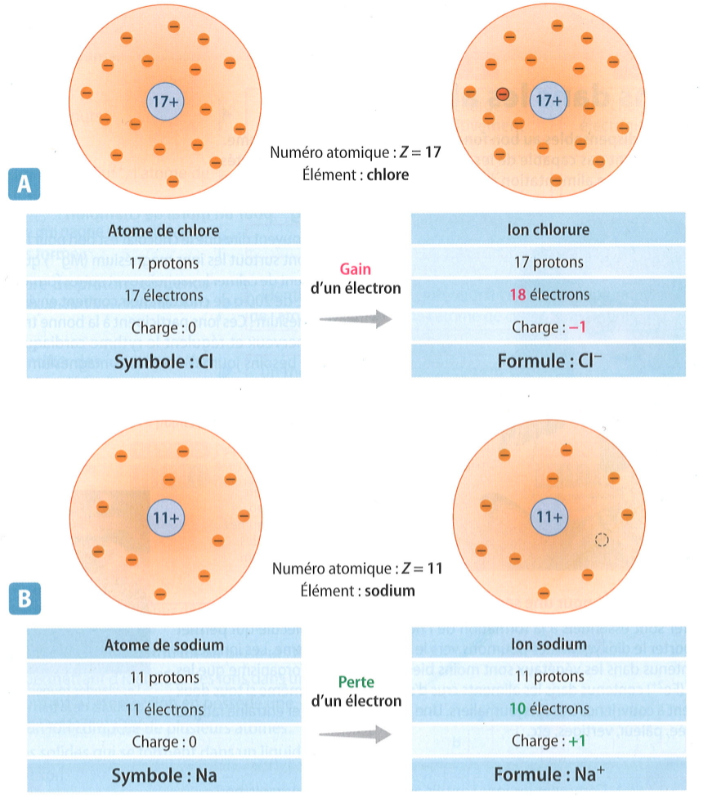
\includegraphics[scale=0.45]{bilan_ions}
%			\end{center}
%		
%%
%\end{frame}

\section{Puissance tension et intensité}



\begin{frame}
\begin{mybilan}
	Pour décrire la vitesse d'un objet en mouvement, on utilise trois caractéristiques :
	\begin{itemize}
		\item la \kw{direction} (horizontale, verticale ou oblique), tangente à la trajectoire;
		
		\item le \kw{sens}, celui du mouvement (vers la gauche, vars la droite, vers le haut etc.);
		
		\item la \kw{valeur} exprimée m/s (ou km/h ou autre).
		
		Si le mouvement est uniforme, la relation \kw{$ v = \dfrac{d}{\Delta t} $}, permet de relier la vitesse de l'objet, la distance parcourue et la durée du parcours avec :
		\begin{itemize}
			\item d : distance parcourue en mètre (m)
			\item $\Delta t$ :durée du trajet en seconde (s)
			\item v : vitesse en mètre par seconde (m/s).
		\end{itemize}
	\end{itemize}



\end{mybilan}


\end{frame}
\section{\'Energie électrique}


\begin{frame}

	\begin{mybilan}
		\begin{itemize}
		\item L'\kw{énergie électrique} utilisée par un appareil de puissance $P$ 	qui fonctionne pendant une durée $t$ est donné par la relation :
		\begin{equation*}
		E = P \times t
		\end{equation*}
		Avec $E$ en kilowattheure (kWh), $P$ en kilowatt (kW) et $t$ en heures (h), ou  $E$ en joules (J), $P$ en watt (W) et $t$ en secondes (s).\pause
		
		%Utiliser des appareil électriques moins puissants, diminuer leur durée de fonctionnement et éviter de les laisser en veille réduit la consommation d'énergie électrique.
		
		
		\item L'énergie électrique fournie par le secteur est \kw{convertie} en un autre type d'énergie suivant l'objet utilisé. \'Energie thermique pour un appareil de chauffage, énergie lumineuse pour une lampe, etc.\pause
		
		\item Toute l'énergie apportée à l'appareil est convertie, il y a \kw{conservation de l'énergie}.
	\end{itemize}
	\end{mybilan}
\end{frame}



\end{document}